\documentclass[9pt,serif,usenames,dvipsnames]{beamer}
\usetheme[progressbar=frametitle]{metropolis}

\useoutertheme{metropolis}
\useinnertheme{metropolis}
\usefonttheme{metropolis}
\usecolortheme{spruce}

\setbeamertemplate{frame numbering}[fraction]
\setbeamercolor{background canvas}{bg=white}
% \setbeamercovered{transparent=15}
\setbeamersize{text margin left=5mm,text margin right=5mm} 
\setbeamertemplate{theorems}[ams style]
\setbeamertemplate{navigation symbols}{}

\setbeamercolor{block body}{bg=mDarkTeal!5}
\setbeamercolor{block title}{bg=mDarkTeal,fg=black!2}
\setbeamercolor{end message}{fg=MSUgreen!60!black, bg=white!85!MSUgreen}


\usepackage{thmtools}
\declaretheorem[style=definition,name=Question]{question}

\usepackage{multicol}
\usepackage{pgfplots}
\usepackage{multicol}
\usepackage{multirow}
\usepackage[export]{adjustbox}
\usepackage{tikz}
\usepackage{xcolor}
\usepackage{xspace}
\usetikzlibrary{arrows,shapes,decorations.pathreplacing,arrows.meta}

\usepackage[linesnumbered,lined,ruled,commentsnumbered]{algorithm2e}
\renewcommand{\algorithmcfname}{ALGORITHM}
\SetAlFnt{\tiny}
\SetAlCapFnt{\tiny}
\SetAlCapNameFnt{\tiny}
%\SetAlCapHSkip{0pt}
%\IncMargin{-\parindent}

\setbeamercolor{block body}{bg=mDarkTeal!5}
\setbeamercolor{block title}{bg=mDarkTeal,fg=black!2}
%\setbeamercolor{end message}{fg=black!2, bg=mDarkTeal}

\usepackage{subcaption}

\usepackage{listings}

\lstset{
	mathescape,
	tabsize=2,
 	framexleftmargin=2mm,
	numbersep=0.5cm,
	%frame=shadowbox,
	basicstyle=\tiny,
	numberstyle=\tiny\color{gray},
	numbers=left,
	backgroundcolor=\color{white},
	escapeinside={(*}{*)},
	rulesepcolor=\color{black}	
	%showtabs=true ,
	%tab=$\dashv$
}

\newcommand{\MyLogo}{\titlegraphic{
\begin{tikzpicture}[overlay, remember picture]
\node[at=(current page.south east), anchor=south east] {%

\includegraphics[width=.2\textwidth]{logo.png}
};
\end{tikzpicture}
}}
\newcommand{\finishes}{\ensuremath{\langle E \rangle}\xspace}
\newcommand{\during}{\ensuremath{\langle D \rangle}\xspace}
\newcommand{\starts}{\ensuremath{\langle B \rangle}\xspace}
\newcommand{\overlaps}{\ensuremath{\langle O \rangle}\xspace}
\newcommand{\meets}{\ensuremath{\langle A \rangle}\xspace}
\newcommand{\before}{\Tlater}
\newcommand{\Tfinishes}{\ensuremath{\langle \overline{E} \rangle}\xspace}
\newcommand{\Tduring}{\ensuremath{\langle \overline{D} \rangle}\xspace}
\newcommand{\Tstarts}{\ensuremath{\langle \overline{B} \rangle}\xspace}
\newcommand{\Toverlaps}{\ensuremath{\langle \overline{O} \rangle}\xspace}
\newcommand{\Tmeets}{\ensuremath{\langle \overline{A} \rangle}\xspace}
\newcommand{\Tbefore}{\later}
\newcommand{\later}{\ensuremath{\langle L \rangle}\xspace}
\newcommand{\Gfinishes}{\ensuremath{[ E ]}\xspace}
\newcommand{\Gduring}{\ensuremath{[ D ]}\xspace}
\newcommand{\Gstarts}{\ensuremath{[ B ]}\xspace}
\newcommand{\Goverlaps}{\ensuremath{[ O ]}\xspace}
\newcommand{\Gmeets}{\ensuremath{[ A ]}\xspace}
\newcommand{\Gbefore}{\TGlater}
\newcommand{\TGfinishes}{\ensuremath{[ \overline{E} ]}\xspace}
\newcommand{\TGduring}{\ensuremath{[ \overline{D} ]}\xspace}
\newcommand{\TGstarts}{\ensuremath{[ \overline{B} ]}\xspace}
\newcommand{\TGoverlaps}{\ensuremath{[ \overline{O} ]}\xspace}
\newcommand{\TGmeets}{\ensuremath{[ \overline{A} ]}\xspace}
\newcommand{\TGbefore}{\Glater}
\newcommand{\Glater}{\ensuremath{[ L ]}\xspace}
\newcommand{\TGlater}{\ensuremath{[ \overline{L} ]}\xspace}
\newcommand{\mmodels}{\ensuremath{\Vdash}}

\newcommand{\len}[2]{\ensuremath{\mathsf{len_{\mathcal{#1} #2}}}}
\newcommand{\lenle}[1]{\ensuremath{\len{\leq}{#1}}}
\newcommand{\lenlt}[1]{\ensuremath{\len{<}{#1}}}
\newcommand{\leneq}[1]{\ensuremath{\len{=}{#1}}}
\newcommand{\lenge}[1]{\ensuremath{\len{\geq}{#1}}}
\newcommand{\lengt}[1]{\ensuremath{\len{>}{#1}}}
\newcommand{\lenne}[1]{\ensuremath{\len{\neq}{#1}}}

\usepackage{array}
\newcolumntype{x}[1]{>{\centering\let\newline\\\arraybackslash\hspace{0pt}}p{#1}}

%\usetikzlibrary{arrows,shapes}

\title[] % (optional, only for long titles)
{\rmfamily\itshape\textbf{Geo-referenced Photo Management System}}

\author[DMSS] % (optional, for multiple authors)
{	
	\textit{Presentation for the Context Aware Systems Project} \hfill\\\\\\\\
	\textbf{Gabriele \textsc{Spina}} \hfill 
}
\MyLogo

\institute[] % (optional)
{
	Università degli Studi di Bologna \\
	Laurea Magistrale in Informatica   \\
}


\date[] % (optional)
{}

\subject{Computer Science}

\begin{document}
\begin{frame}[plain, noframenumbering]
\titlepage
\end{frame}

\section{Introduction}
\MyLogo

\begin{frame}
\MyLogo
\frametitle{Photos Geo-Localization}
\begin{center}
\begin{columns}

	\begin{column}{.5\textwidth}
	\begin{itemize}
		\item The geo-localization of the photos is a functional information 
		\item The usage of geo-localization in the construction of a photo management system can significantly improve the quality of the service offered
	\end{itemize} 
	\end{column}

	\begin{column}{.5\textwidth}
	\begin{figure}
	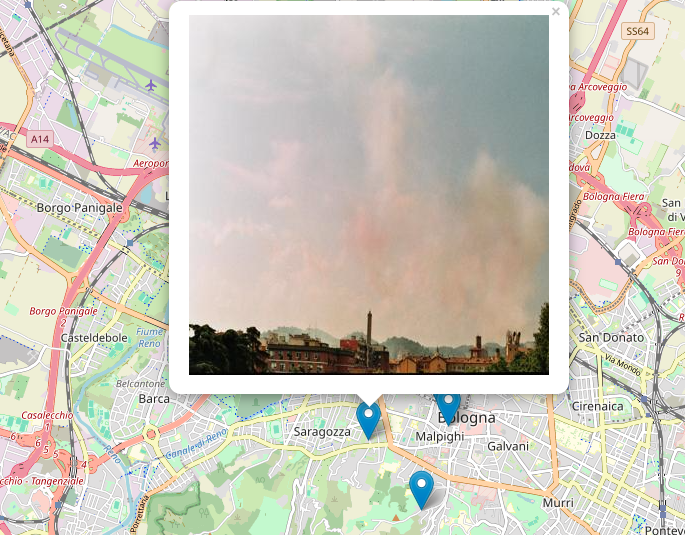
\includegraphics[width= \textwidth]{marker_opened.png}	
	\caption{Example: visualize photos as markers on the map with the possibility to click on the marker to see the related photo}
	\end{figure}
	\end{column}
\end{columns}
\end{center}
\end{frame}

\begin{frame}
\MyLogo
\frametitle{Proposed Solution}

\begin{center}
	\begin{itemize}
		\item In this work a geo-referenced photo management system is constructed
		\item A spatial database is implemented to store and retrieve the data
		\item There is a mobile application from which the user can take photos and visualize them 
		\item The feature of visualizing photos on the map, as in the image in the previous slide, is implemented in a web dashboard
		\end{itemize}
\end{center}

\end{frame}

\section{Spatial Database}
\begin{frame}
\MyLogo
\frametitle{PostgreSQL}

\begin{center}
\begin{columns}

	\begin{column}{.5\textwidth}
	\begin{itemize}
		\item The spatial database is implemented using the PostgreSQL database management system 
		\item The database is composed of two tables: one for photos and one for the referring collection
	\end{itemize} 
	\end{column}

	\begin{column}{.5\textwidth}
	\begin{table}[h!]
\centering
\begin{tabular}{llll}
\multicolumn{4}{c}{Media Files}                                            \\ \hline
\multicolumn{2}{l|}{id}             & \multicolumn{2}{l}{serial}           \\
\multicolumn{2}{l|}{name}           & \multicolumn{2}{l}{varchar}          \\
\multicolumn{2}{l|}{date}           & \multicolumn{2}{l}{timestamp}        \\
\multicolumn{2}{l|}{image}          & \multicolumn{2}{l}{bytea}            \\
\multicolumn{2}{l|}{position}       & \multicolumn{2}{l}{geography(point)} \\
\multicolumn{2}{l|}{collection\_id} & \multicolumn{2}{l}{int}             
\end{tabular}
\caption{Media files table design.}
\label{table:mf}
\end{table}

\begin{table}[h!]
\centering
\begin{tabular}{llll}
\multicolumn{4}{c}{Collections}                                     \\ \hline
\multicolumn{2}{l|}{collection\_id} & \multicolumn{2}{l}{serial}    \\
\multicolumn{2}{l|}{name}           & \multicolumn{2}{l}{varchar}   \\
\multicolumn{2}{l|}{created\_at}    & \multicolumn{2}{l}{timestamp}
\end{tabular}
\caption{Collections table design.}
\label{table:col}
\end{table}

	\end{column}
\end{columns}
\end{center}

\end{frame}	

\section{Mobile Application}
\begin{frame}
\MyLogo
\frametitle{Mobile Gallery}

\begin{center}
\begin{columns}

	\begin{column}{.5\textwidth}
	\begin{itemize}
\item The application is a simple gallery, from which images in different collections can be visualized
\item Implemented using Kivy library with Python language
\item There is the possibility to take a new photo and save it in a collection
\item Then, other features, like the creation of a new collection or the retrieval of the photos taken nearest to the user position
\end{itemize}
	\end{column}

	\begin{column}{.5\textwidth}
	\begin{figure}
	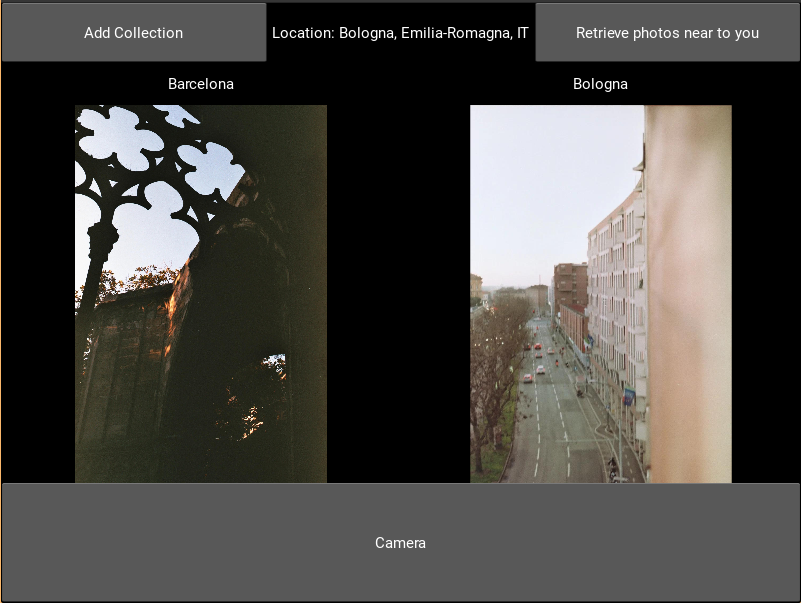
\includegraphics[width= \textwidth]{app.png}	
	\caption{Mobile Gallery, main screen}
	\end{figure}
	\end{column}
\end{columns}
\end{center}

\end{frame}

\section{Web Dashboard}
\begin{frame}
\MyLogo
\frametitle{Visualize Photos on Map}

With the mobile application there is not the possibility to visualize photos on map, or even to upload more photos at once; a web dashboard is constructed to overcome these issues and provide more features.
\begin{itemize}
\item The frontend is implemented with Leaflet, JavaScript, HTML; the data received from the backend is visualized on the map on the basis of user's actions 
\item The backend is implemented with Flask and Python; the requests received from the frontend are satisfied by querying the database and manipulating data, according to the particular request

\end{itemize}
\end{frame}

\begin{frame}
\MyLogo
\frametitle{Web Dashboard Features}

\begin{center}
The web dashboard (on the right) offers the possibility to interact with photos in different ways:

\begin{columns}
	\begin{column}{.5\textwidth}
	\begin{itemize}
\item \textbf{Photo Upload}: single photo or folder, with the possibility to apply spatial perturbation to the saving position for folder case
\item \textbf{GeoJson Upload}: upload a file containing zones definition, filter photos by zones
\item \textbf{Cluster and HeatMap}: cluster all photos in groups, visualize photos in a heatmap
\item \textbf{Chronological Path}: build a path reconstructing the road crossed from various photos
\item \textbf{Gallery}: visualize all collections and photos
\end{itemize}
	\end{column}

	\begin{column}{.5\textwidth}
	\begin{figure}
	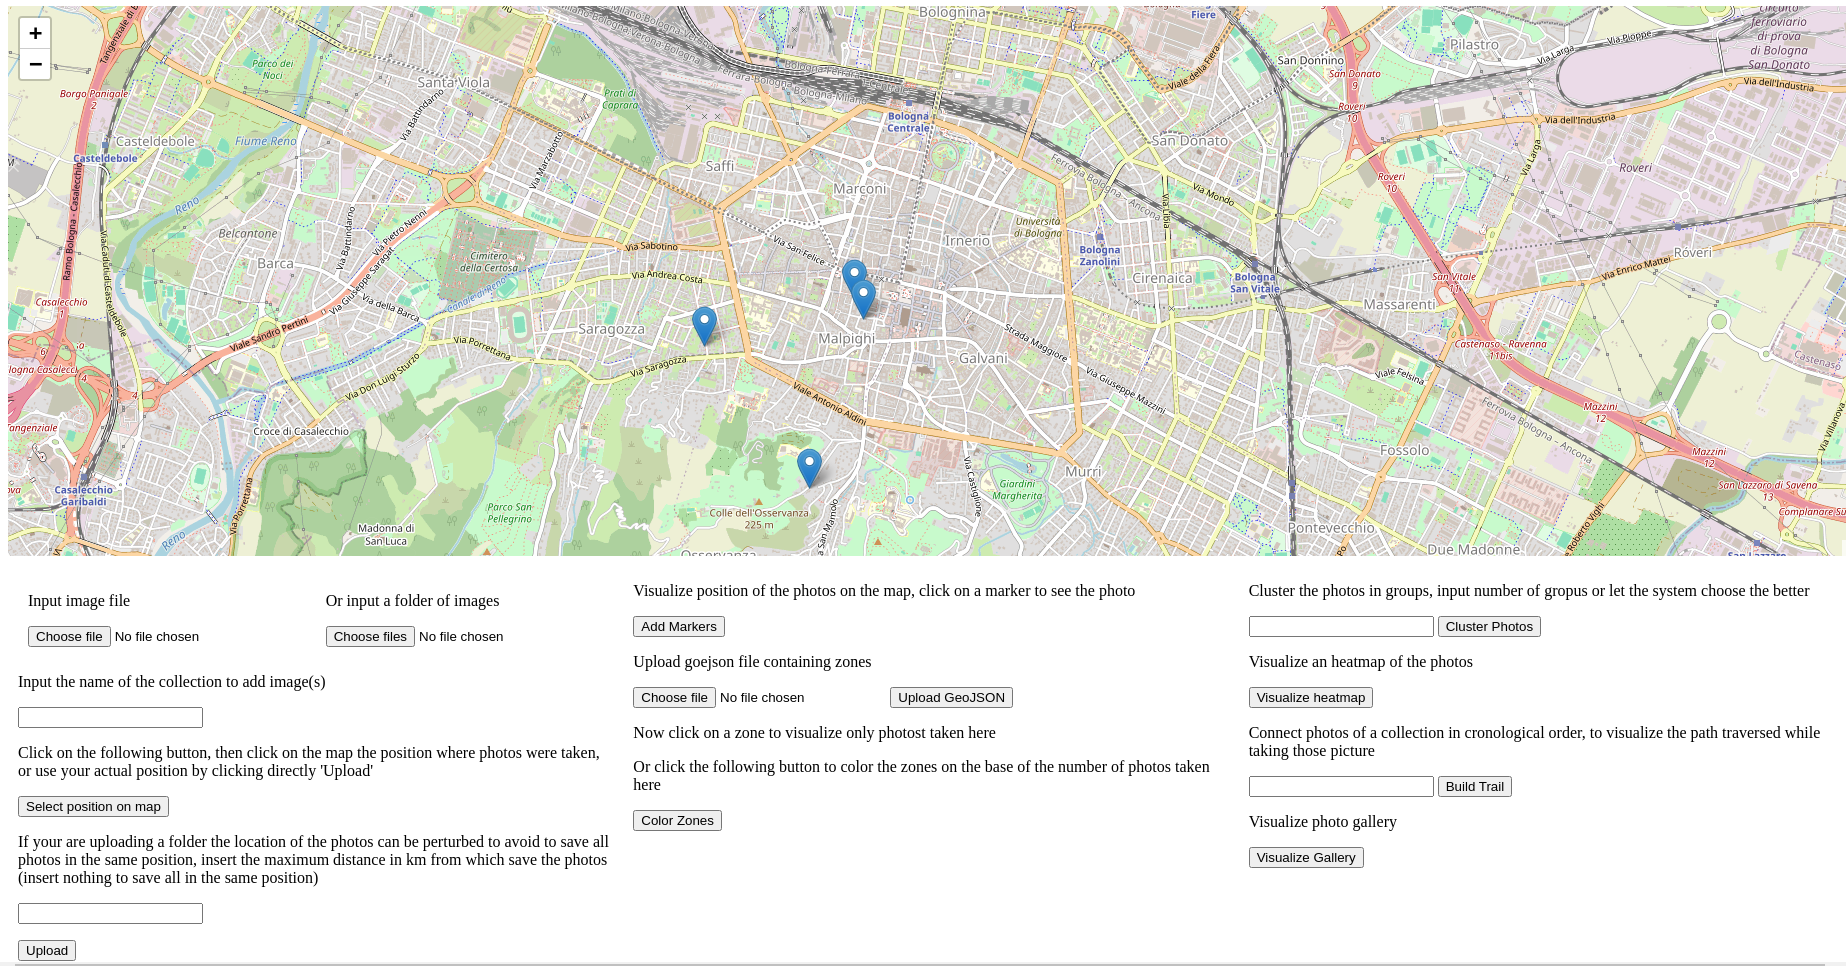
\includegraphics[width= \textwidth]{dash.png}	
	\caption{Web Dashboard, main screen}
	\end{figure}
	\end{column}
\end{columns}
\end{center}

\end{frame}

\section{Conclusion}
\begin{frame}
\MyLogo
\frametitle{Conclusion}

\begin{itemize}
\item The system works well in a local environment with a small amount of data. 
\item The scalability of the system with large amounts of data is not so good, mainly because the photos are stored directly in the database
\item To improve that, photos could be stored in a cloud and then referred in the database with the link
\end{itemize}

\end{frame}

\begin{frame}[plain]
\vfill \vfill \vfill \vfill \vfill \vfill \vfill \vfill
\begin{beamercolorbox}[sep=1.0cm, center, shadow=false, rounded=false]{end message}
\begin{huge}
Thanks for your attention!
\end{huge}
\\
Now a demo of the system...
\end{beamercolorbox}

\vfill \vfill \vfill \vfill \vfill \vfill \hfill

\includegraphics[width=.12\textwidth, right]{logo.png}

\end{frame}

\end{document}